\documentclass[]{tufte-handout}

% ams
\usepackage{amssymb,amsmath}

\usepackage{ifxetex,ifluatex}
\usepackage{fixltx2e} % provides \textsubscript
\ifnum 0\ifxetex 1\fi\ifluatex 1\fi=0 % if pdftex
  \usepackage[T1]{fontenc}
  \usepackage[utf8]{inputenc}
\else % if luatex or xelatex
  \makeatletter
  \@ifpackageloaded{fontspec}{}{\usepackage{fontspec}}
  \makeatother
  \defaultfontfeatures{Ligatures=TeX,Scale=MatchLowercase}
  \makeatletter
  \@ifpackageloaded{soul}{
     \renewcommand\allcapsspacing[1]{{\addfontfeature{LetterSpace=15}#1}}
     \renewcommand\smallcapsspacing[1]{{\addfontfeature{LetterSpace=10}#1}}
   }{}
  \makeatother

\fi

% graphix
\usepackage{graphicx}
\setkeys{Gin}{width=\linewidth,totalheight=\textheight,keepaspectratio}

% booktabs
\usepackage{booktabs}

% url
\usepackage{url}

% hyperref
\usepackage{hyperref}

% units.
\usepackage{units}


\setcounter{secnumdepth}{-1}

% citations


% pandoc syntax highlighting

% table with pandoc

% multiplecol
\usepackage{multicol}

% strikeout
\usepackage[normalem]{ulem}

% morefloats
\usepackage{morefloats}


% tightlist macro required by pandoc >= 1.14
\providecommand{\tightlist}{%
  \setlength{\itemsep}{0pt}\setlength{\parskip}{0pt}}

% title / author / date
\title{Conociendo Rstudio}
\author{Jorge Meneses \and Paulo Peña}
\date{}


\begin{document}

\maketitle




Rstudio es la principal aplicación para usar R. En esta sesión
empezaremos por conocer la interface y como podemos utilizarla.

\hypertarget{paneles-clave-rstudio}{%
\section{Paneles Clave RStudio}\label{paneles-clave-rstudio}}

Rstudio tiene los siguientes 4 paneles o áreas claves:

\begin{itemize}
\tightlist
\item
  Source Code o Editor de Código es la fuente donde escribes tú código.
  La información escrita puede ser luego almacenada, modificada y
  compartida con otros usuarios.
\item
  Console o Consola donde se presenta los resultados de las operaciones
  que comandamos en el guión.
\item
  El ambiente o Environment donde almacenamos los objetos que vamos
  creando como tablas, bases de datos o funciones.
\item
  Files/Plots/Packages/Help, donde puedes ver tus archivos de la
  computadora, gráficos, paquetes (esto lo veremos luego) y archivos de
  ayuda.
\end{itemize}

\hypertarget{source-codeeditor-de-cuxf3digo}{%
\subsection{Source Code/Editor de
Código}\label{source-codeeditor-de-cuxf3digo}}

Done se crea y edita los códigos de R. Aunque esrtos archivos se guardan
con la extensión ``.R'', estos solo son archivos de texto. Los
resultados del código se verán en el panel de Consola.

El guión cuenta el número de línea donde se está escribiend el código.
Para escribir anotaciones en el guión, se debe anteceder la línea con el
símbolo ``\#''. También se puede dividir el guión secciones con
``\#\#\#\#\#'' haciéndo más fácil la navegación dentro del guión.

El editor de código será nuestro principal espacio de trabajo. Aquí
podemos escribir todas las instrucciones para realizar nuestros análisis
y reportes.

El guión se puede ejecutar por líneas o completo. Si solo quiere
ejecutar unas líneas, se debe seleccionar las líneas deseadas y apretar
el botón Enter o también en el extremos derecho del panel se encuentra
la opción ``Run''. Si se desea ejecutar todo un guión, en el extremos
derecho del panel se selecciona la opción ``Source''.

\begin{figure}
\includegraphics[width=17.78in]{../../public/img/02 - Guión R} \caption[Guión R]{Guión R}\label{fig:unnamed-chunk-2}
\end{figure}

\hypertarget{consola}{%
\subsection{Consola}\label{consola}}

La consola de R es el área donde se presentan los resultados del código
que hemos ejecutado. Si hay algún error en el código escrito, la consola
nos indicará sobre dicho error. Existen diferentes tipos de errores,
pueden ser desde algo simple como un signo de puntuación mal puesto
hasta cosas más complejas como falta de archivos en la computadora.

Adicionalmente, también se puede colocar líneas de código directa en la
consola y el programa ejecutará los comandos, sin embargo, estas líneas
de códigos no serán grabadas.

\begin{marginfigure}
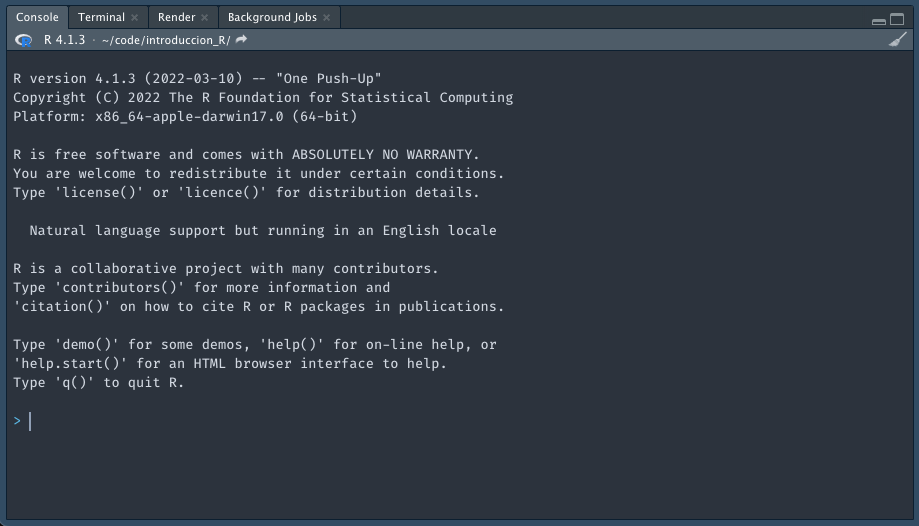
\includegraphics[width=12.76in]{../../public/img/02 - consola R} \caption[Consola R]{Consola R}\label{fig:unnamed-chunk-3}
\end{marginfigure}

\hypertarget{ambiente-o-environment}{%
\subsection{Ambiente o Environment}\label{ambiente-o-environment}}

\begin{marginfigure}
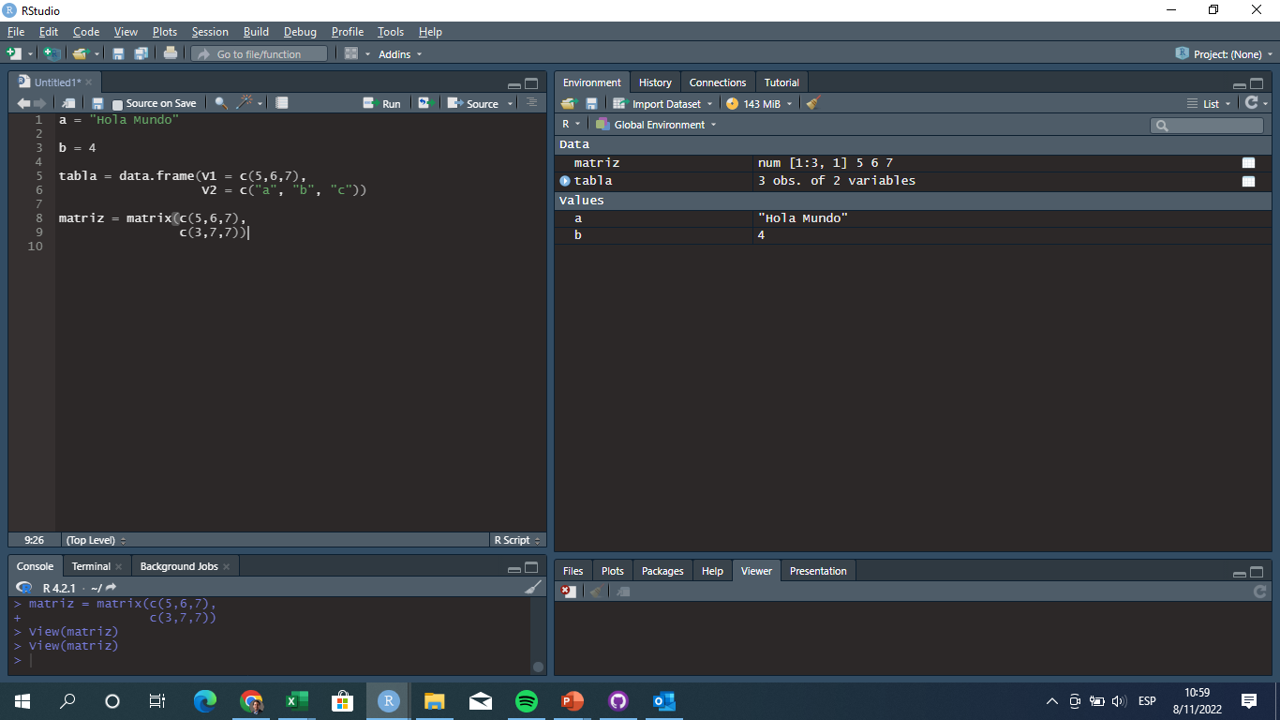
\includegraphics[width=17.78in]{../../public/img/02 - environment} \caption[Editor de código]{Editor de código}\label{fig:unnamed-chunk-4}
\end{marginfigure}

\hypertarget{el-panel-de-ayuda-gruxe1ficos-plots-archivos}{%
\subsection{El panel de ayuda, gráficos (plots),
archivos}\label{el-panel-de-ayuda-gruxe1ficos-plots-archivos}}

\hypertarget{tipo-de-variables-en-rstudio}{%
\section{Tipo de Variables en
RStudio}\label{tipo-de-variables-en-rstudio}}

Creación de variables

Tarea: un guión con un conjunto de variables, una de cada tipo



\end{document}
